%!TEX root = paper.tex

To analyze the 1-dimensional problem, we will derive two groups of sequences from the original collision sequence, which we will call the $\beta$ and $\delta$ groups. These group will allow us to validate any collision sequence. The first sequence in the $\beta$ group is defined below.

\begin{definition}
	Given a collision sequence $\alpha$, define a sequence $\beta^{(0)}$ such that each element $\beta^{(0)}_i$ is the number of h's between the $i^{th}$ and $(i+1)^{th}$ v in $\alpha$. From Lemma \ref{lem:interval-ticks}, each element in $\beta^{(0)}$ can be one of two different values, which we will refer to as $\beta^{(0)}_{min}, \beta^{(0)}_{max}$.
\end{definition}

Graphically, $\beta^{(0)}_i$ represents the number of tick marks in each interval. An example of this is shown in Figure \ref{fig:beta-sequence}.

\begin{figure}[H]
  \begin{center}
    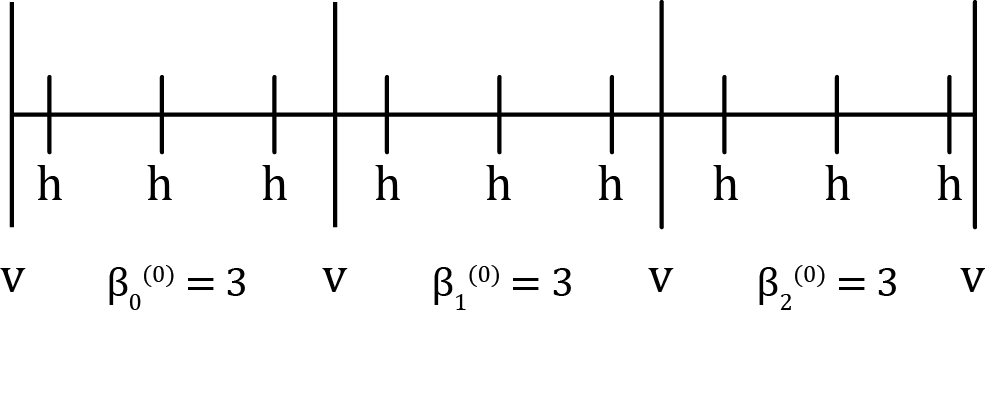
\includegraphics[keepaspectratio]{1d_mapping_3}
  \end{center}
  \vspace{-.2in} % corrects bad spacing
  \caption{\label{fig:beta-sequence} An example $\beta^{(0)}$ sequence.}
\end{figure}

The first sequence in the $\delta$ group, $\delta^{(0)}$, is defined such that each element is spaced $\cbracket{\frac{m}{1}}$ apart. $\delta^{(0)}$ will also include an offset of $-(1-y_0)$ for reasons that will become clear shortly. In terms of our $\beta$ group, $\cbracket{\frac{m}{1}}$ can be written as 

\begin{equation}
  \cbracket{\frac{m}{1}} = \frac{m}{1} - \beta^{(0)}_{min}
\end{equation}

\begin{definition}
  Given a $\beta^{(0)}$ sequence, $\delta^{(0)}$ is defined as follows

  \begin{align}\label{delta_beta}
    \delta^{(0)}_i \coloneqq \begin{cases}
      -(1-y_0) \qquad &\text{for} \quad i = 0\\
      i (m - \beta^{(0)}_{min}) - (1-y_0) \qquad &\text{for} \quad i \ge 1
    \end{cases}
  \end{align}
\end{definition}

Visually, each element $\delta^{(0)}_i$ is the distance between the beginning of the $i^{th}$ interval and the $(i \, \beta^{(0)}_{min})^{th}$ tick mark (with positive distance measured right to left). Figure \ref{fig:delta-sequence} shows the $\delta^{(0)}_i$ sequence on top of the original parametric representation (top of the Figure) as well as by itself (bottom of the Figure).

\begin{figure}[H]
  \begin{center}
    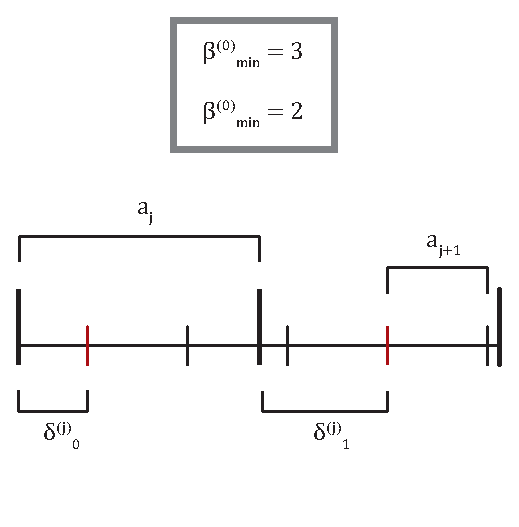
\includegraphics[keepaspectratio]{1d_mapping_4}
  \end{center}
  \vspace{-.2in} % corrects bad spacing
  \caption{\label{fig:delta-sequence} Generating the $\delta^{(0)}$ sequence.}
\end{figure}

Our next step is to define $\beta^{(j)}, \delta^{(j)}$ for $j \ge 1$, which will be done in an inductive manner. Before continuing, let's create a new sequence that will be helpful for defining the rest of the $\beta$ and $\delta$ groups.

\begin{definition}
  Assume that the $\beta$ group is fully defined, then $a$ is defined as follows

  \begin{equation}
    a_j \coloneqq \begin{cases}
      m \qquad &\text{for} \quad i = -2\\
      1 \qquad &\text{for} \quad i = -1\\
      a_{j-2} - \beta^{(j)}_{min} a_{j-1} \qquad &\text{for} \quad i \ge 0
    \end{cases}
  \end{equation}
\end{definition}

$a_{-2}, a_{-1}$ are the interval size and tick spacing in our original problem. $a_0$ is the spacing of elements of $\delta^{(0)}$, which is illustrated in Figure \ref{fig:a-0}.

\begin{figure}[H]
  \begin{center}
    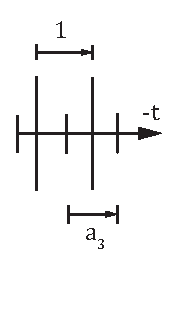
\includegraphics[keepaspectratio]{1d_mapping_5}
  \end{center}
  \vspace{-.2in} % corrects bad spacing
  \caption{\label{fig:a-0} $a_0$.}
\end{figure}

$\delta^{(j)}$ will be defined such that the spacing of elements of the sequences will be $a_j$ for $j \ge 1$. For the moment, the reader should assume that, given some $j$, then $\delta^{(j-1)}$ exists and its elements are strictly increasing and evenly spaced. An example $\delta^{(j-1)}$ sequence is shown in Figure \ref{fig:delta-sequence-2}.

\begin{figure}[H]
  \begin{center}
    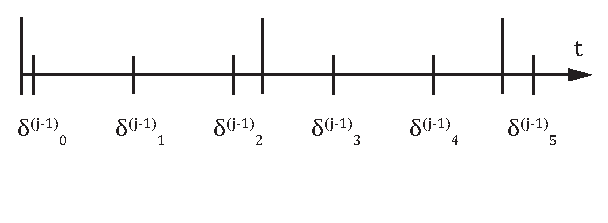
\includegraphics[keepaspectratio]{1d_mapping_6}
  \end{center}
  \vspace{-.2in} % corrects bad spacing
  \caption{\label{fig:delta-sequence-2} An example $\delta^{(j-1)}$ sequence.}
\end{figure}

\begin{definition}
  \label{def:beta-definition}
  Given a collision sequence $\alpha$, for some $j > 0$ assume that $\beta^{(j-1)}$ is defined and each element in the sequence is either $\beta^{(j-1)}_{min}$ or $\beta^{(j-1)}_{max}$. The sequence $\beta^{(j)}$ is defined such that each element $\beta^{(j)}_i$ is 1 more than the number of occurrences of $\beta^{(j-1)}_{min}$ between the $i^{th}$ and $(i+1)^{th}$ occurrence of $\beta^{(j-1)}_{max}$ in the $\beta^{(j-1)}$ sequence. From Lemma \ref{lem:interval-ticks}, each element in $\beta^{(j)}$ can be one of two different values, which we will refer to as $\beta^{(j)}_{min}, \beta^{(j)}_{max}$.

  If, for some $j_f$, the length of $\beta^{(j_f-1)}$ is 1, then $\beta^{(j_f-1)}$ is called the terminating $\beta$ sequence, and all subsequent $\beta^{(j)}$ for $j \ge j_f$ are undefined.
\end{definition}

$\beta^{(j)}$ is much simpler to understand visually. Let's return to the example $\delta^{(j-1)}$ sequence, shown in Figure \ref{fig:delta-sequence-2}. We need to understand how the $\delta^{(j-1)}$ sequence is related to the $\beta^{(j-1)}$ sequence. 

Referring back to Figure \ref{fig:delta-sequence}, it can be seen that $\beta^{(j-1)}_i$ is equal to $\beta^{(j-1)}_{min}$ plus the number of tick marks included in the $\delta^{(j-1)}_{i+1}$ interval minus the number of tick marks included in the $\delta^{(j-1)}_i$ interval. More precisely

\begin{align}\label{eq:beta_i}
  \beta^{(j-1)}_i = \floor{\delta^{(j-1)}_{i+1}} + \beta^{(j)}_{min} - \floor{\delta^{(j-1)}_i} 
\end{align}

Figure \ref{fig:beta-sequence-j} plots the $\beta^{(j-1)}$ sequence in place of the $\delta^{(j)}$ sequence. Reffering back to the definition of $\beta^{(j)}$, it can be seen that $\beta^{(j)}$ counts the number of tick marks in each interval on the $\delta^{(j-1)}$ plot.

\begin{figure}[H]
  \begin{center}
    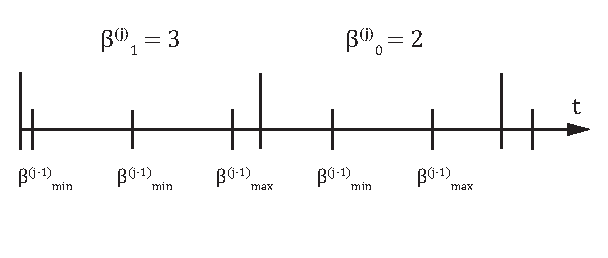
\includegraphics[keepaspectratio]{1d_mapping_7}
  \end{center}
  \vspace{-.2in} % corrects bad spacing
  \caption{\label{fig:beta-sequence-j} A general $\beta^{(j)}$ sequence.}
\end{figure}

As was promised earlier, we will finish defining the $\delta$ group. In words, each $\delta^{(j)}_i$ is the distance between the beginning of the $i^{th}$ interval and the $(i \, \beta^{(j)}_{min})^{th}$ tick mark in the $\beta^{(j)}$ visual representation.

\begin{definition}
  $\delta^{(j)}$ is defined more precisely as

  \begin{align}\label{delta_beta}
    \delta^{(j)}_i \coloneqq \begin{cases}
      1(1-y_0) \qquad &\text{for} \quad i = 0\\
      i (a_{j-2} - \beta^{(j)}_{min} * a_{j-1}) - (1-y_0) \qquad &\text{for} \quad i \ge 1
    \end{cases}
  \end{align}
\end{definition}


